\section{Patch Generation}
\label{sec:patch-gen}

Figure~\ref{overview-fixing} outlines the fixing process. While the
steps of parsing and tree-based representation learning are the same
as in~train\-ing, the step of applying the trained CCL and CTL to
produce the candidate patches is different. Figure~\ref{fig:patch-gen}
shows that step.

\begin{figure}[t]
	\centering
	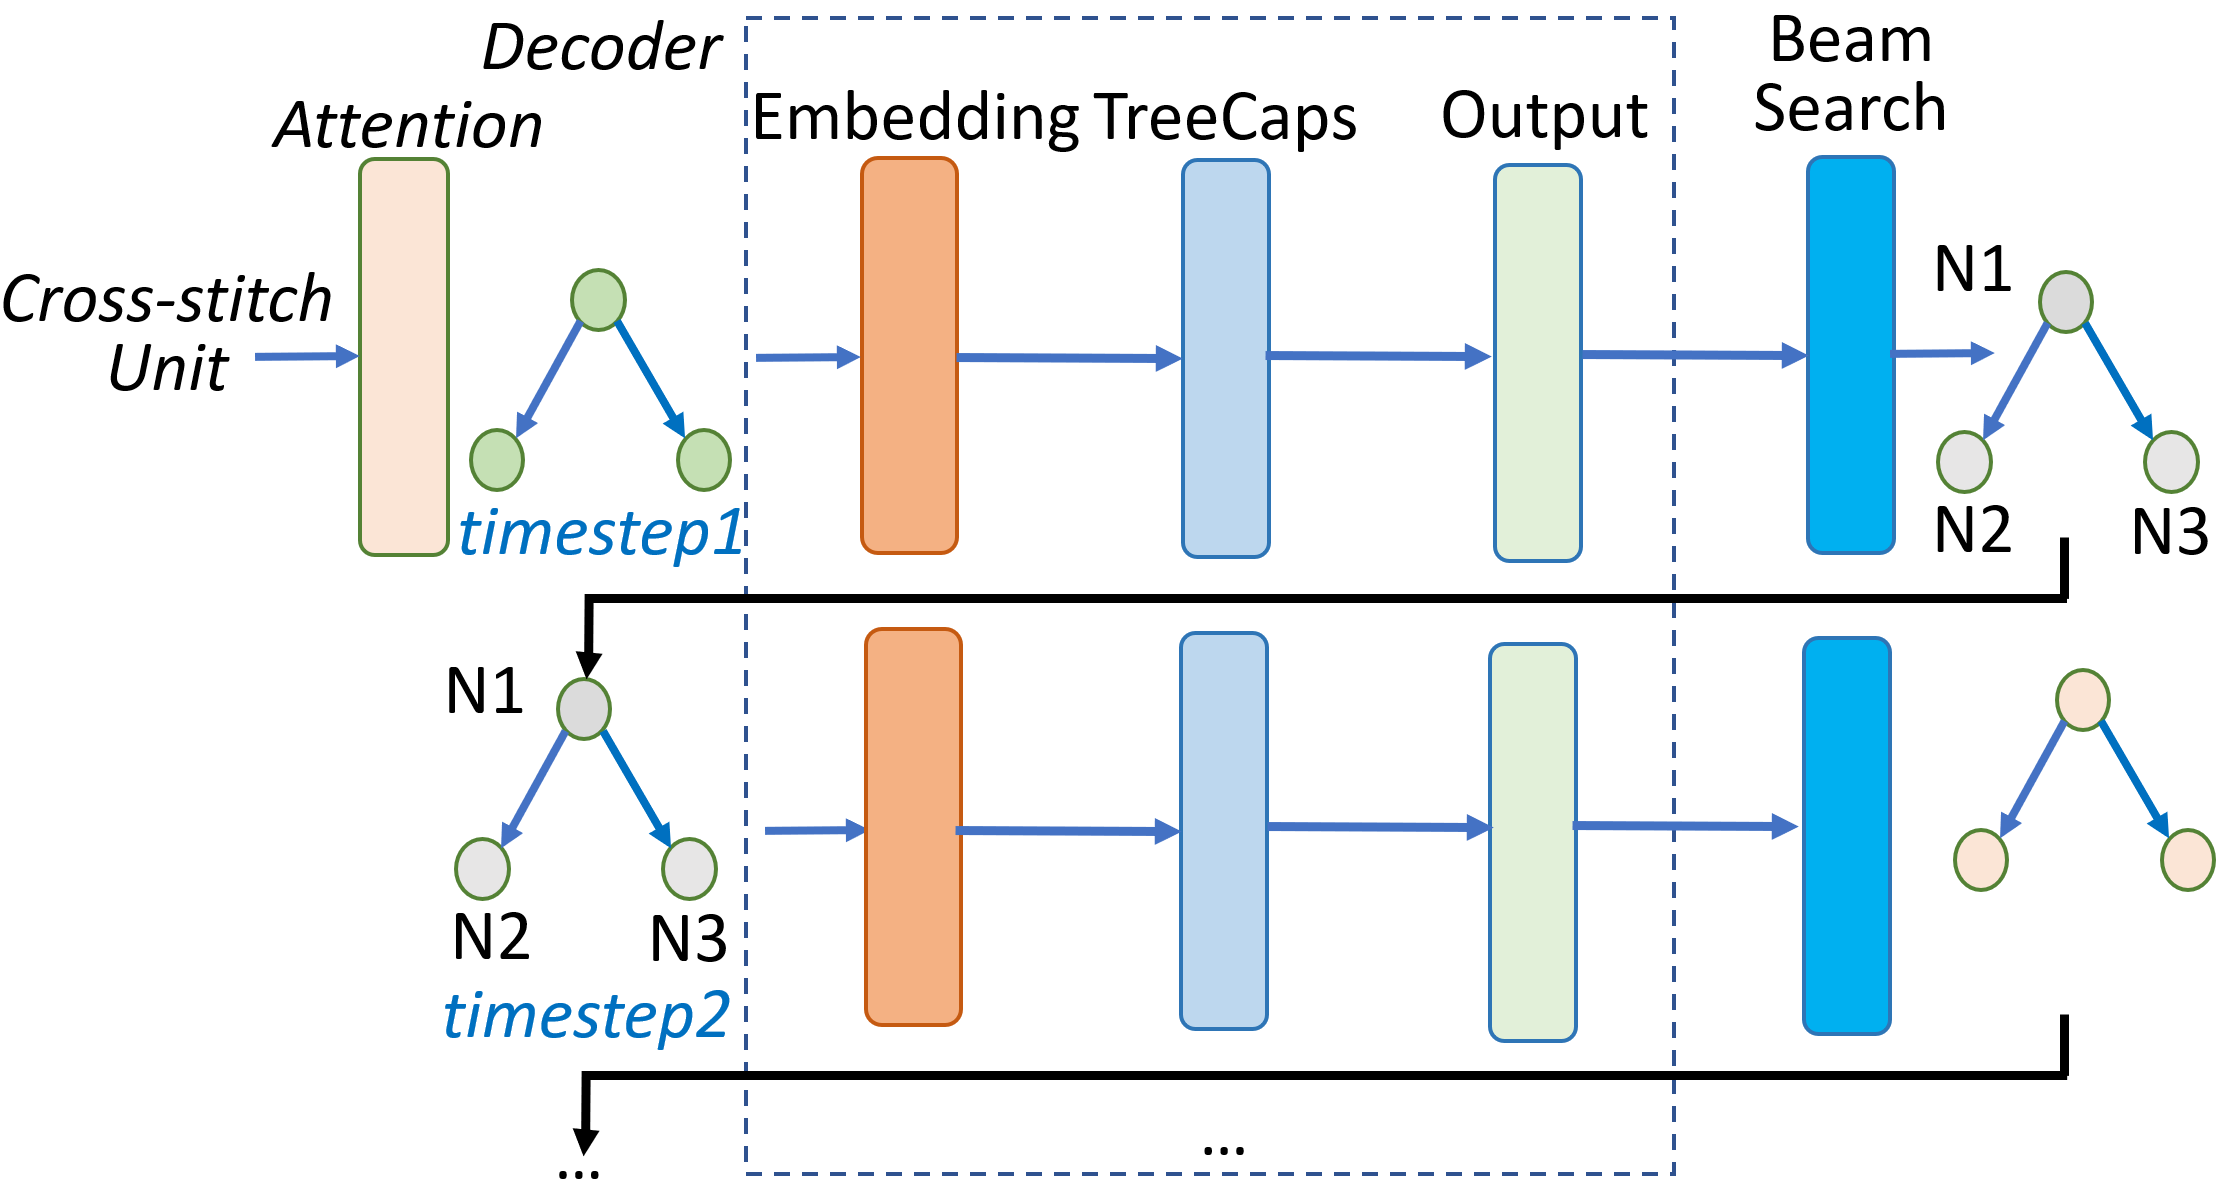
\includegraphics[width=2.9in]{graphs/beam-search.png}
        \vspace{-10pt}
	\caption{Patch Generation via Tree-Structured Beam Search}
	\label{fig:patch-gen}
\end{figure}

%As explained earlier in Figure~\ref{fig:dual-learning},
The output of the cross-stitch unit connects to the attention layer,
which in turn connects to the decoder. The decoder has four main
components (Figure~\ref{fig:patch-gen}): 1) the embedding component to
encode the input at a time step into the subtree whose nodes are
vectors; 2) the TreeCaps~\cite{bui2021treecaps} component to summarize
the vectors in a subtree into a vector; 3) the output layer; and 4)
the beam search component, which takes the output at the output layer
and produces a candidate patch (at the current time step $i$) in terms
of the output AST subtree $T_i$ with the concrete source code for the
AST nodes. While the embedding component, TreeCaps, and the output
layer are straightforward, let us explain the adaptation in the beam
search component.

Beam search is an optimization strategy to keep only the top-$K$ best
solution for the output subtree $T_i$ at a time step $i$ to help
reduce the search space. We need to use a beam search
strategy because at each node when we convert a vector back to a code
token, we might have multiple candidate tokens for each node. For
example, in Figure~\ref{fig:patch-gen}, we might have multiple
candidates for $N_1$, $N_2$, and $N_3$.
%Thus, we might face the combinatorial explosion when considering a
%potential large number of nodes in the output subtree $T_i$ at each
%time step $i$.

Because the beam search component aims to produce the subtree
in which some of its nodes will be used in the tree-based convolutional
window as the input of the decoder at the next time step $i+1$
(Figure~\ref{fig:patch-gen}), it must work in accordance with 
TreeCaps. TreeCaps computes the vector from bottom up (i.e.,
the vectors for children nodes are computed before the one for their
parent node). Therefore, our beam search component considers the order
of the nodes in the AST subtree from the bottom-up order, and then the
left-to-right order of the sibling nodes of the same parent node. For
example, for the tree $V1$--$V5$ in Figure~\ref{overview-training},
the beam search component will consider the order of the nodes as
follows: $V2$, $V4$, $V5$, $V3$, and $V1$. The sequences of code
tokens in that order for the AST nodes are considered. The score for a
sequence is the product of the probabilities of all the nodes. At each
step, the sequences are ranked and only the top-$K$ best sequences are
maintained.

Another issue occurs during the conversion from an embedding to a code
token. When we search in our dictionary for a token that has a vector
closest to the vector of the current node, we
might encounter a token that is not in the same project or invalid for
the current scope of the program. Thus, we perform static analysis
with several filters to keep only the valid tokens in the current
scope. Specifically, we apply a set of filters to verify the program
semantics as in DLFix~\cite{icse20}. We use the alpha-renaming filter
to change the names back to Java code using a dictionary
containing all the valid names in the scope, the syntax-checking
filter to remove the candidates with syntax errors, and the name
validation filter to check the validity of the variables, methods, and
classes.
Afterward, we run the corresponding test cases for the current
bug. If there is any test case failed, {\tool} attempts the next
candidate.
%If all test cases pass, we regards the candidate as correct.

%The first problem is that when transferring the predicted fixing to
%the real tokens, beam search uses the GloVe embedding
%dictionary. However, this dictionary is learned from multiple
%projects. So the invalid tokens may be generated by the beam
%search. So \tool creates a rule that before using the beam search,
%\tool firstly makes static analysis to select all appeared token in
%the project and when doing the beam search, the results only come from
%the appeared token set.

%Secondly, because the beam search is designed for sequential data,
%\tool makes some small changes to work on the tree structure. To be
%more detailed, \tool regards the nodes with the same parent node as
%the same level. And when doing the beam search, \tool considers these
%nodes at one time by multiply the possibility score for each node. The
%beam search order is from the bottom to the top, which means the node
%with a higher height will be considered first.

%For example, in Figure \ref{patch-validation}, the AST node $N3$ and
%$N4$ will be considered the first when doing beam search. If the
%possibility of $N3=Dataset$ is $p_1$ and the possibility of $N4=null$
%is $p_2$. The first step of beam search will have an optimal token
%like $N3=Dataset, N4=null$ with the possibility of $p_1*p_2$. The
%second step of the beam search is to search $N2$ and $N5$ in the dark
%box simultaneously. And the last step of the beam search is dealing
%with the node $N1$ in the orange box.


%This step will only be used during the prediction, and because the statement-level program repair is our main goal for the dual learning, \tool only consider the output from the statement-level here. After \tool has the predicted fixing for the subtree of AST $Tree_s$, \tool uses the beam search to help the model reduce the search space and run the test cases to do the validation. Beam search is an optimized greedy strategy, and Beam search keeps only the $n$ optimal tokens for each step to help reduce the search space. However, there are two problems the beam search may face when applying to \tool to do the validation.





%After doing the beam search, \tool runs the corresponding test cases for the bug $b_i$. If there is any test case failed, \tool tries the second candidate for the fixing. If all test cases passed, \tool regards the current candidate as the correct fixing for the bug $b_i$, which is the final output for the \tool.


